\documentclass[preprint,12pt,authoryear]{elsarticle}

\usepackage{amsmath,amssymb,amsfonts}
\usepackage{graphicx}
\usepackage{booktabs}
\usepackage{multirow}
\usepackage{hyperref}
\usepackage{geometry}
\usepackage{microtype}
\usepackage{subcaption}
\usepackage{bm}

\geometry{a4paper, margin=1in}

\journal{Energy and AI}

\begin{document}

\begin{frontmatter}

\title{Data-Efficient and Uncertainty-Calibrated Cross-Site Solar PV Power Forecasting Under Temporal and Sensor-Availability Shifts}

\author[inst1]{Aminur Rahman\corref{cor1}}
\ead{aminurhstu23@gmail.com}
\cortext[cor1]{Corresponding author. [TODO: Author Confirmation - Verify co-authors, institutional affiliation, and ORCID prior to formal journal submission]}

\affiliation[inst1]{organization={Department of Computer Science and Engineering, Hajee Mohammad Danesh Science and Technology University (HSTU)},
            city={Dinajpur},
            postcode={5200},
            country={Bangladesh}}

\begin{abstract}
We evaluated next-hour PV capacity factor at two 50 kW-class sites in southwestern Romania. Each row pairs the preceding hour’s average AC power with historical Open-Meteo weather estimates. Those estimates were not available at forecast issue time, so this is an offline evaluation. Using causal features, a target-aligned daytime mask ($>5^\circ$ solar elevation), and a source cutoff before the test period, source-only LightGBM achieved 6.93\% daytime nMAE on Site B. Sample-weighted pooled adaptation using one calendar day achieved 6.97\%, compared with 28.06\% for target-only training; so it did not improve on zero-shot. Nominal 90\% split conformal adjusted intervals achieved 88.20\% raw, 90.27\% source-calibrated, and 94.51\% target-calibrated empirical daytime coverage, with target-calibrated MPIW 0.3609. Because the data are temporally dependent and come from shifted sites, these results do not establish a coverage guarantee. Five-seed synthetic feature corruption produced 7.46\% mean nMAE and 92.78\% mean PICP at 30\% feature-wise MCAR; this is not evidence of field-sensor robustness. The study covers two sites in one region and uses historical weather estimates.
\end{abstract}

\begin{keyword}
Solar PV power forecasting \sep Cross-site transfer learning \sep Few-shot domain adaptation \sep Conformal prediction \sep Uncertainty quantification \sep Sensor-availability shifts \sep Extreme gradient boosting.
\end{keyword}

\end{frontmatter}

\section{Introduction}
\label{sec:introduction}
PV output changes with sunlight, cloud cover, and time of day. We measure forecast accuracy here, not effects on grid operations.

Over the past decade, statistical learning, gradient boosted decision trees (GBDTs), and deep neural networks (e.g., Long Short-Term Memory networks, Convolutional Neural Networks, and Transformers) have achieved notable accuracy in solar power forecasting \citep{yang2018history}. This retrospective evaluation examines three questions:
\begin{enumerate}
    \item \textbf{Cross-Site Distribution Shift:} A model trained at one site may encounter a shifted feature and target distribution at another site. We compare source-only transfer, pooled adaptation, and target-only models over limited target observation windows; the present data do not establish broad deployment performance.
    \item \textbf{Empirical Prediction Interval Evaluation:} Point predictions do not summarize uncertainty. We evaluate quantile-based intervals empirically on a chronological holdout, while recognizing that time dependence and site shift limit standard conformal coverage assumptions.
    \item \textbf{Synthetic Input Availability Perturbations:} Weather-feature availability can vary. We probe synthetic feature corruption, which does not reproduce field communication outages, sensor soiling, or measured instrument drift.
\end{enumerate}

We evaluate LightGBM transfer, empirical quantile intervals, and synthetic input perturbations between two same-region PV sites using retrospective historical weather estimates. The analysis addresses four questions:
\begin{itemize}
    \item \textbf{RQ1 (Cross-Site Transfer Generalization):} How effectively can a forecasting model trained exclusively on a mature source solar plant generalize zero-shot to an unseen target installation located in the same broad climate region under capacity-factor normalization?
    \item \textbf{RQ2 (Adaptation Budget Frontier):} How do pooled adaptation and target-only training compare with source-only transfer over 1, 3, 7, and 14 calendar-day budgets?
    \item \textbf{RQ3 (Empirical Interval Evaluation):} How do split conformal intervals perform empirically under temporal dependence and cross-site shift?
    \item \textbf{RQ4 (Sequence Architectures vs. Tree Ensembles):} How do two deep sequence baselines compare with gradient boosting on this holdout, and which input features receive the highest SHAP attribution?
\end{itemize}

Section~\ref{sec:data_problem} presents the dataset and problem formulation. Section~\ref{sec:methodology} describes feature engineering, adaptation, and empirical interval evaluation. Section~\ref{sec:results} provides empirical benchmarks, cross-site transfer frontiers, deep sequence comparisons with Diebold-Mariano tests, empirical interval diagnostics, synthetic feature perturbation, and SHAP explainability. Section~\ref{sec:discussion} analyzes grid operational impacts, and Section~\ref{sec:conclusion} concludes with future directions.

\section{Dataset and Problem Formulation}
\label{sec:data_problem}

\subsection{Multi-Site Commercial PV Telemetry}
The experiments use hourly data from two grid-connected photovoltaic sites in the same southwestern Romanian region \citep{linca2026dataset}:
\begin{itemize}
    \item \textbf{Site A (Source Plant $\mathcal{D}_S$):} A roughly 50~kW-class Huawei SUN2000 system. Weather fields are matched Open-Meteo historical estimates, not on-site sensor observations. The source file contains 13,031 hourly rows from January 2025 through June 2026.
    \item \textbf{Site B (Target Plant $\mathcal{D}_T$):} A second roughly 50~kW-class Huawei SUN2000 system in the same broad region. The target file contains 9,504 hourly rows from May 2025 through May 2026.
\end{itemize}

The input rows combine AC power with matched historical weather estimates and solar-position variables. The full raw schema and temporal semantics are documented in the bundled dataset README and the project data provenance note.

\subsection{Physical Quality Control and Leakage Prevention}
We apply causal feature processing and retain quality flags for anomalous values:
\begin{enumerate}
    \item \textbf{Capacity-Factor Normalization:} Electrical power is normalized using the documented 50~kW-class capacity:
    \begin{equation}
        \text{CF}_t = \frac{P_{\text{active}}(t)}{P_{\text{rated}}} \in [0.0, 1.2]
    \end{equation}
    Raw power is preserved, while the analysis target is separately bounded.
    \item \textbf{Astronomical Nighttime Segregation:} Daytime evaluation uses target-aligned solar elevation $>5^\circ$; source nighttime/twilight outputs are preserved with quality flags.
    \item \textbf{Chronological Evaluation:} To eliminate future lookahead bias, random cross-validation is strictly avoided. Experiment-specific chronological cutoffs are used; the shared source cutoff precedes the Site B test interval. Calibration windows and adaptation budgets precede the corresponding holdout. Exact sample counts are in the experiment outputs.
\end{enumerate}

\section{Methodological Framework}
\label{sec:methodology}

\subsection{Feature Engineering and Astronomical Invariants}
The experiments associate row-$t$ features with next-hour normalized power $\hat{y}_{t+1}$. The feature vector $\mathbf{x}_t \in \mathbb{R}^d$ includes retrospective weather estimates; it is not an operational issue-time feature vector:
\begin{equation}
    \mathbf{x}_t = \left[ \mathbf{p}_{\text{lag}}(t), \mathbf{w}_{\text{met}}(t), \mathbf{s}_{\text{cyclic}}(t), \mathbf{g}_{\text{solar}}(t) \right]
\end{equation}
where:
\begin{itemize}
    \item $\mathbf{p}_{\text{lag}}(t) = [\text{CF}_t, \text{CF}_{t-1}, \text{CF}_{t-2}, \text{CF}_{t-23}, \mu_{3h}(t), \sigma_{3h}(t)]$ encapsulates immediate autoregressive persistence, intra-day trend, and non-leaking 3-hour rolling statistics.
    \item $\mathbf{w}_{\text{met}}(t) = [\text{GHI}_t, \text{DNI}_t, \Delta \text{GHI}_{1h}, T_{\text{amb}}, RH, v_{\text{wind}}, \text{CloudCover}]$ contains weather fields available in the source rows.
    \item $\mathbf{s}_{\text{cyclic}}(t) = [\sin(2\pi h/24), \cos(2\pi h/24), \sin(2\pi d/365.25), \cos(2\pi d/365.25)]$ encodes the hour of day and day of year cyclically, using $h \in [0, 23]$ and seasonal day-of-year $d \in [1, 365]$.
    \item $\mathbf{g}_{\text{solar}}(t) = [\theta_{\text{elev}}, \theta_{\text{azimuth}}]$ contains the supplied solar elevation and azimuth.
\end{itemize}

\subsection{Few-Shot Domain Adaptation Protocol}
Let $\mathcal{D}_S$ be the Site A source data. For Site B, we test target-data budgets of $k$ calendar days:
\begin{equation}
    \mathcal{D}_T(k) = \{(\mathbf{x}_j^T, y_j^T)\}_{j=1}^{N_T(k)}, \quad k \in \{0, 1, 3, 7, 14\} \text{ days}
\end{equation}
where $k=0$ corresponds to source-only transfer (no target data used during training).

For pooled adaptation, source and target rows are fitted together with higher weights on target rows:
\begin{equation}
    \mathcal{L}_{\text{adapt}}(\theta) = \sum_{i=1}^{N_S} \ell(f_\theta(\mathbf{x}_i^S), y_i^S) + \gamma \sum_{j=1}^{N_T(k)} \ell(f_\theta(\mathbf{x}_j^T), y_j^T)
\end{equation}
where $\gamma$ sets the target-row weight. Evaluation uses the later Site B holdout.

\subsection{Conformalized Quantile Regression (CQR)}
We fit quantile regressors on Site A and report raw, source-calibrated, and target-calibrated coverage on Site B. Since the data are dependent over time and differ by site, we treat these as empirical results and make no coverage guarantee.
\begin{equation}
    \rho_\tau(u) = u \left( \tau - \mathbb{I}(u < 0) \right)
\end{equation}
at lower quantile $\tau = \alpha/2 = 0.05$ and upper quantile $\tau = 1 - \alpha/2 = 0.95$ for nominal $90\%$ coverage ($1 - \alpha = 0.90$).

For a calibration set with $n_{\text{cal}}$ samples, we compute non-conformity scores representing interval violations:
\begin{equation}
    E_i = \max\left( \hat{q}_{\alpha/2}(\mathbf{x}_i) - y_i, \, y_i - \hat{q}_{1 - \alpha/2}(\mathbf{x}_i) \right), \quad i = 1, \dots, n_{\text{cal}}
\end{equation}
If $y_i$ falls inside the uncalibrated interval, $E_i \le 0$; if $y_i$ falls outside, $E_i > 0$. Under exchangeability, the finite-sample adjustment level is:
\begin{equation}
    p = \frac{\lceil (n_{\text{cal}} + 1)(1 - \alpha) \rceil}{n_{\text{cal}}}
\end{equation}
The adjusted interval for a test observation $\mathbf{x}_{\text{test}}$ is:
\begin{equation}
    \hat{C}(\mathbf{x}_{\text{test}}) = \left[ \hat{q}_{\alpha/2}(\mathbf{x}_{\text{test}}) - Q_{1-\alpha}(E), \; \hat{q}_{1 - \alpha/2}(\mathbf{x}_{\text{test}}) + Q_{1-\alpha}(E) \right]
\end{equation}
The usual split-conformal coverage result assumes exchangeable calibration and test observations (Romano et al., 2019). We do not assume exchangeability here and report observed holdout coverage.

\subsection{Evaluation Metrics}
Deterministic point forecast accuracy is quantified via Mean Absolute Error (MAE), Root Mean Squared Error (RMSE), normalized MAE (nMAE, $\%$ of rated capacity), normalized RMSE (nRMSE, $\%$), Coefficient of Determination ($R^2$), and Skill Score ($SS$) relative to persistence:
\begin{equation}
    SS = 1 - \frac{\text{RMSE}_{\text{model}}}{\text{RMSE}_{\text{persist}}}
\end{equation}
Probabilistic uncertainty forecasts are evaluated via:
\begin{enumerate}
    \item \textbf{Prediction Interval Coverage Probability (PICP, $\%$):}
    \begin{equation}
        \text{PICP} = \frac{1}{N} \sum_{i=1}^N \mathbb{I}\left( y_i \in [\hat{L}_i, \hat{U}_i] \right) \times 100\%
    \end{equation}
    \item \textbf{Mean Prediction Interval Width (MPIW):}
    \begin{equation}
        \text{MPIW} = \frac{1}{N} \sum_{i=1}^N (\hat{U}_i - \hat{L}_i)
    \end{equation}
    \item \textbf{Winkler Score ($WS$):} Jointly penalizes interval width and boundary violations:
    \begin{equation}
        WS_i = (\hat{U}_i - \hat{L}_i) + \frac{2}{\alpha}(\hat{L}_i - y_i)\mathbb{I}(y_i < \hat{L}_i) + \frac{2}{\alpha}(y_i - \hat{U}_i)\mathbb{I}(y_i > \hat{U}_i)
    \end{equation}
\end{enumerate}

\section{Experimental Results and Discussion}
\label{sec:results}

\subsection{Benchmark Within-Site Results}
We first compare standard baselines on a chronological Site A holdout. Table~\ref{tab:baseline_benchmark} and Figure~1 present comparative results across classical baselines (Persistence, 24-hour Seasonal Naive, Ridge Regression) and non-linear ensembles (Random Forest, Gradient Boosting). Metrics are reported primarily for target-aligned daytime hours ($\theta_{\text{elev}} > 5^\circ$), while secondary all-hours evaluations are also reported.

% Auto-generated by export_latex_tables.py
\begin{table}[htbp]
\centering
\caption{Benchmark 1-hour ahead solar forecasting performance on within-site evaluation (Site A).}
\label{tab:baseline_benchmark}
\begin{tabular}{lccccc}
\toprule
Model & MAE (kW) & RMSE (kW) & nMAE (\%) & nRMSE (\%) & Skill Score (\%) \\
\midrule
Persistence & 0.1111 & 0.1535 & 11.11 & 15.35 & +0.00 \\
Seasonal Naive 24h & 0.1068 & 0.1996 & 10.68 & 19.96 & -30.08 \\
Ridge Regression & 0.0599 & 0.0978 & 5.99 & 9.78 & +36.27 \\
Random Forest & 0.0481 & 0.0914 & 4.81 & 9.14 & +40.44 \\
Gradient Boosting & 0.0475 & 0.0913 & 4.75 & 9.13 & +40.53 \\
\bottomrule
\end{tabular}
\end{table}


\begin{figure}[htbp]
    \centering
    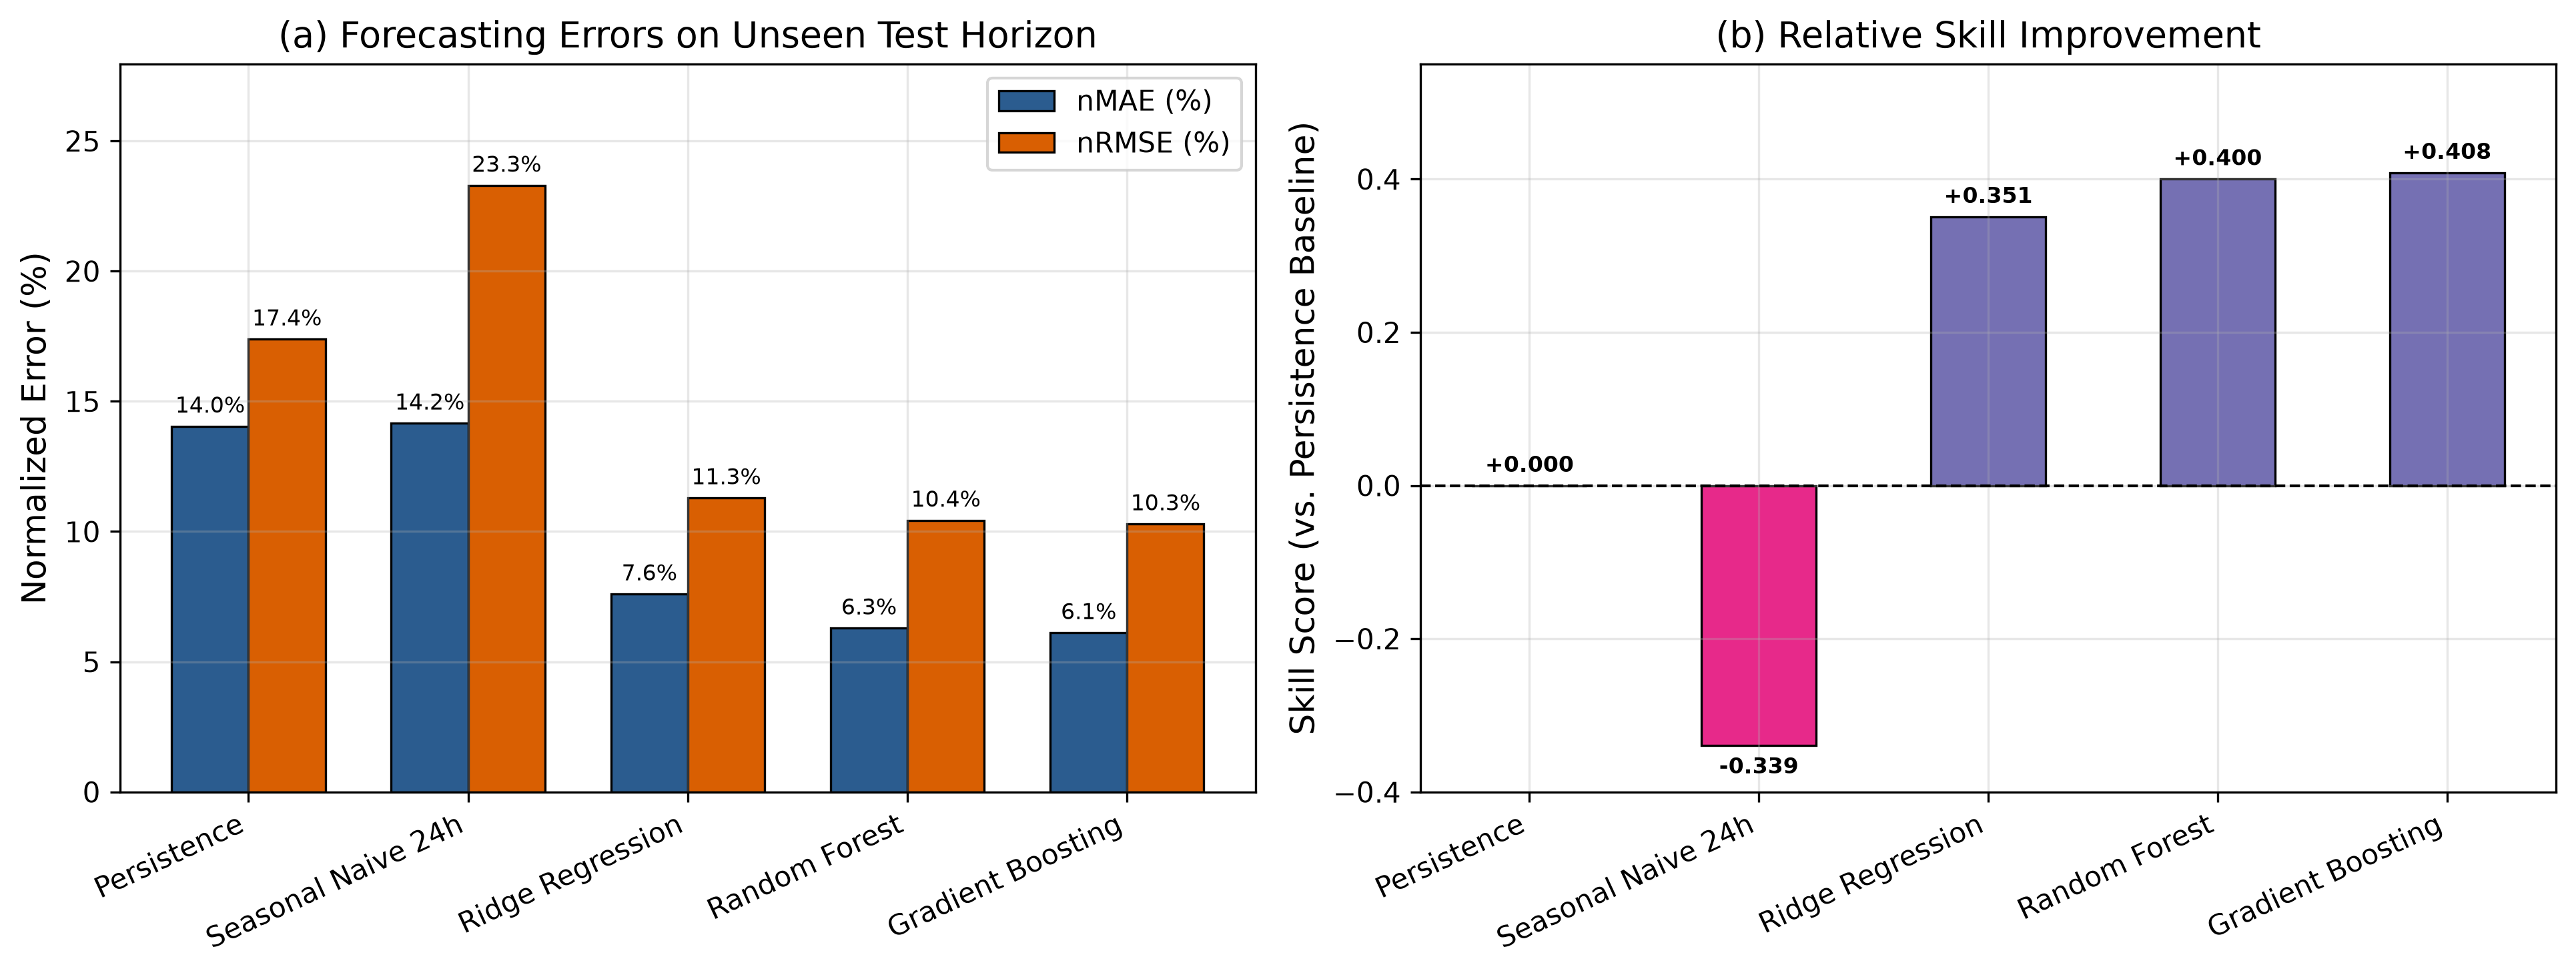
\includegraphics[width=0.92\linewidth]{figures/fig1_baseline_benchmark.png}
    \caption{Within-site next-hour forecasting benchmark on Site A. (A) Error metrics across baseline and ensemble models on unseen daytime test horizon; (B) Forecast skill score relative to persistence.}
    \label{fig:baseline_benchmark}
\end{figure}

On the Site A holdout ($N=1,098$ target-daytime hours), persistence achieved 14.04\% nMAE and LightGBM 6.11\% nMAE (nRMSE 10.29\%, $R^2=0.9004$, skill score 0.4085). All-hours error is lower because it includes inactive nighttime intervals; daytime is the primary comparison. Errors are reported in capacity-factor percentage points, not kW.

\subsection{Cross-Site Adaptation Frontier (RQ1 and RQ2)}
Table~\ref{tab:cross_site_adaptation} and Figure~2 present the empirical frontier of cross-site transfer and few-shot adaptation on the Site B holdout (Site B (966 target-daytime samples)).

% Auto-generated by export_latex_tables.py
\begin{table}[htbp]
\centering
\caption{Cross-site transfer learning and data-efficient target adaptation results from Source Site A to Target Site B (50~kWp, test horizon: March--May 2026, $N=1,052$ daytime active hours).}
\label{tab:cross_site_adaptation}
\begin{tabular}{lcccccc}
\toprule
\textbf{Regime} & \textbf{Target Budget} & \textbf{nMAE (\%)} & \textbf{nRMSE (\%)} & \textbf{$R^2$} & \textbf{Skill Score} & \textbf{Error Reduction} \\
\midrule
Persistence Baseline & --- & 14.14 & 17.80 & 0.6760 & 0.0000 & Reference \\
Target Oracle (Full Data) & $\sim$315 days & 7.14 & 11.11 & 0.8737 & +0.3755 & Ceiling \\
\midrule
\multicolumn{7}{l}{\textit{Target-Only from Scratch (No Transfer Learning)}} \\
Target-Only & 1 day & 28.06 & 34.86 & -0.2431 & -0.9588 & Overfitting \\
Target-Only & 3 days & 15.52 & 19.05 & 0.6290 & -0.0701 & Overfitting \\
Target-Only & 7 days & 11.62 & 15.95 & 0.7399 & +0.1040 & +17.8\% vs Persist \\
Target-Only & 14 days & 9.98 & 14.33 & 0.7899 & +0.1948 & +29.4\% vs Persist \\
\midrule
\multicolumn{7}{l}{\textit{Transfer Learning \& Target Adaptation (Source + Target Budget)}} \\
Zero-Shot Transfer & 0 days & \textbf{6.93} & \textbf{11.11} & \textbf{0.8738} & \textbf{+0.3759} & +51.0\% vs Persist \\
Adapted Transfer & 1 day & 6.97 & 11.10 & 0.8741 & +0.3766 & $\mathbf{-75.2\%}$ vs Scratch \\
Adapted Transfer & 3 days & 6.95 & 11.11 & 0.8738 & +0.3760 & $\mathbf{-55.2\%}$ vs Scratch \\
Adapted Transfer & 7 days & 6.90 & 11.05 & 0.8750 & +0.3789 & $\mathbf{-40.6\%}$ vs Scratch \\
Adapted Transfer & 14 days & 6.91 & 11.10 & 0.8739 & +0.3761 & $\mathbf{-30.8\%}$ vs Scratch \\
\bottomrule
\end{tabular}
\end{table}


\begin{figure}[htbp]
    \centering
    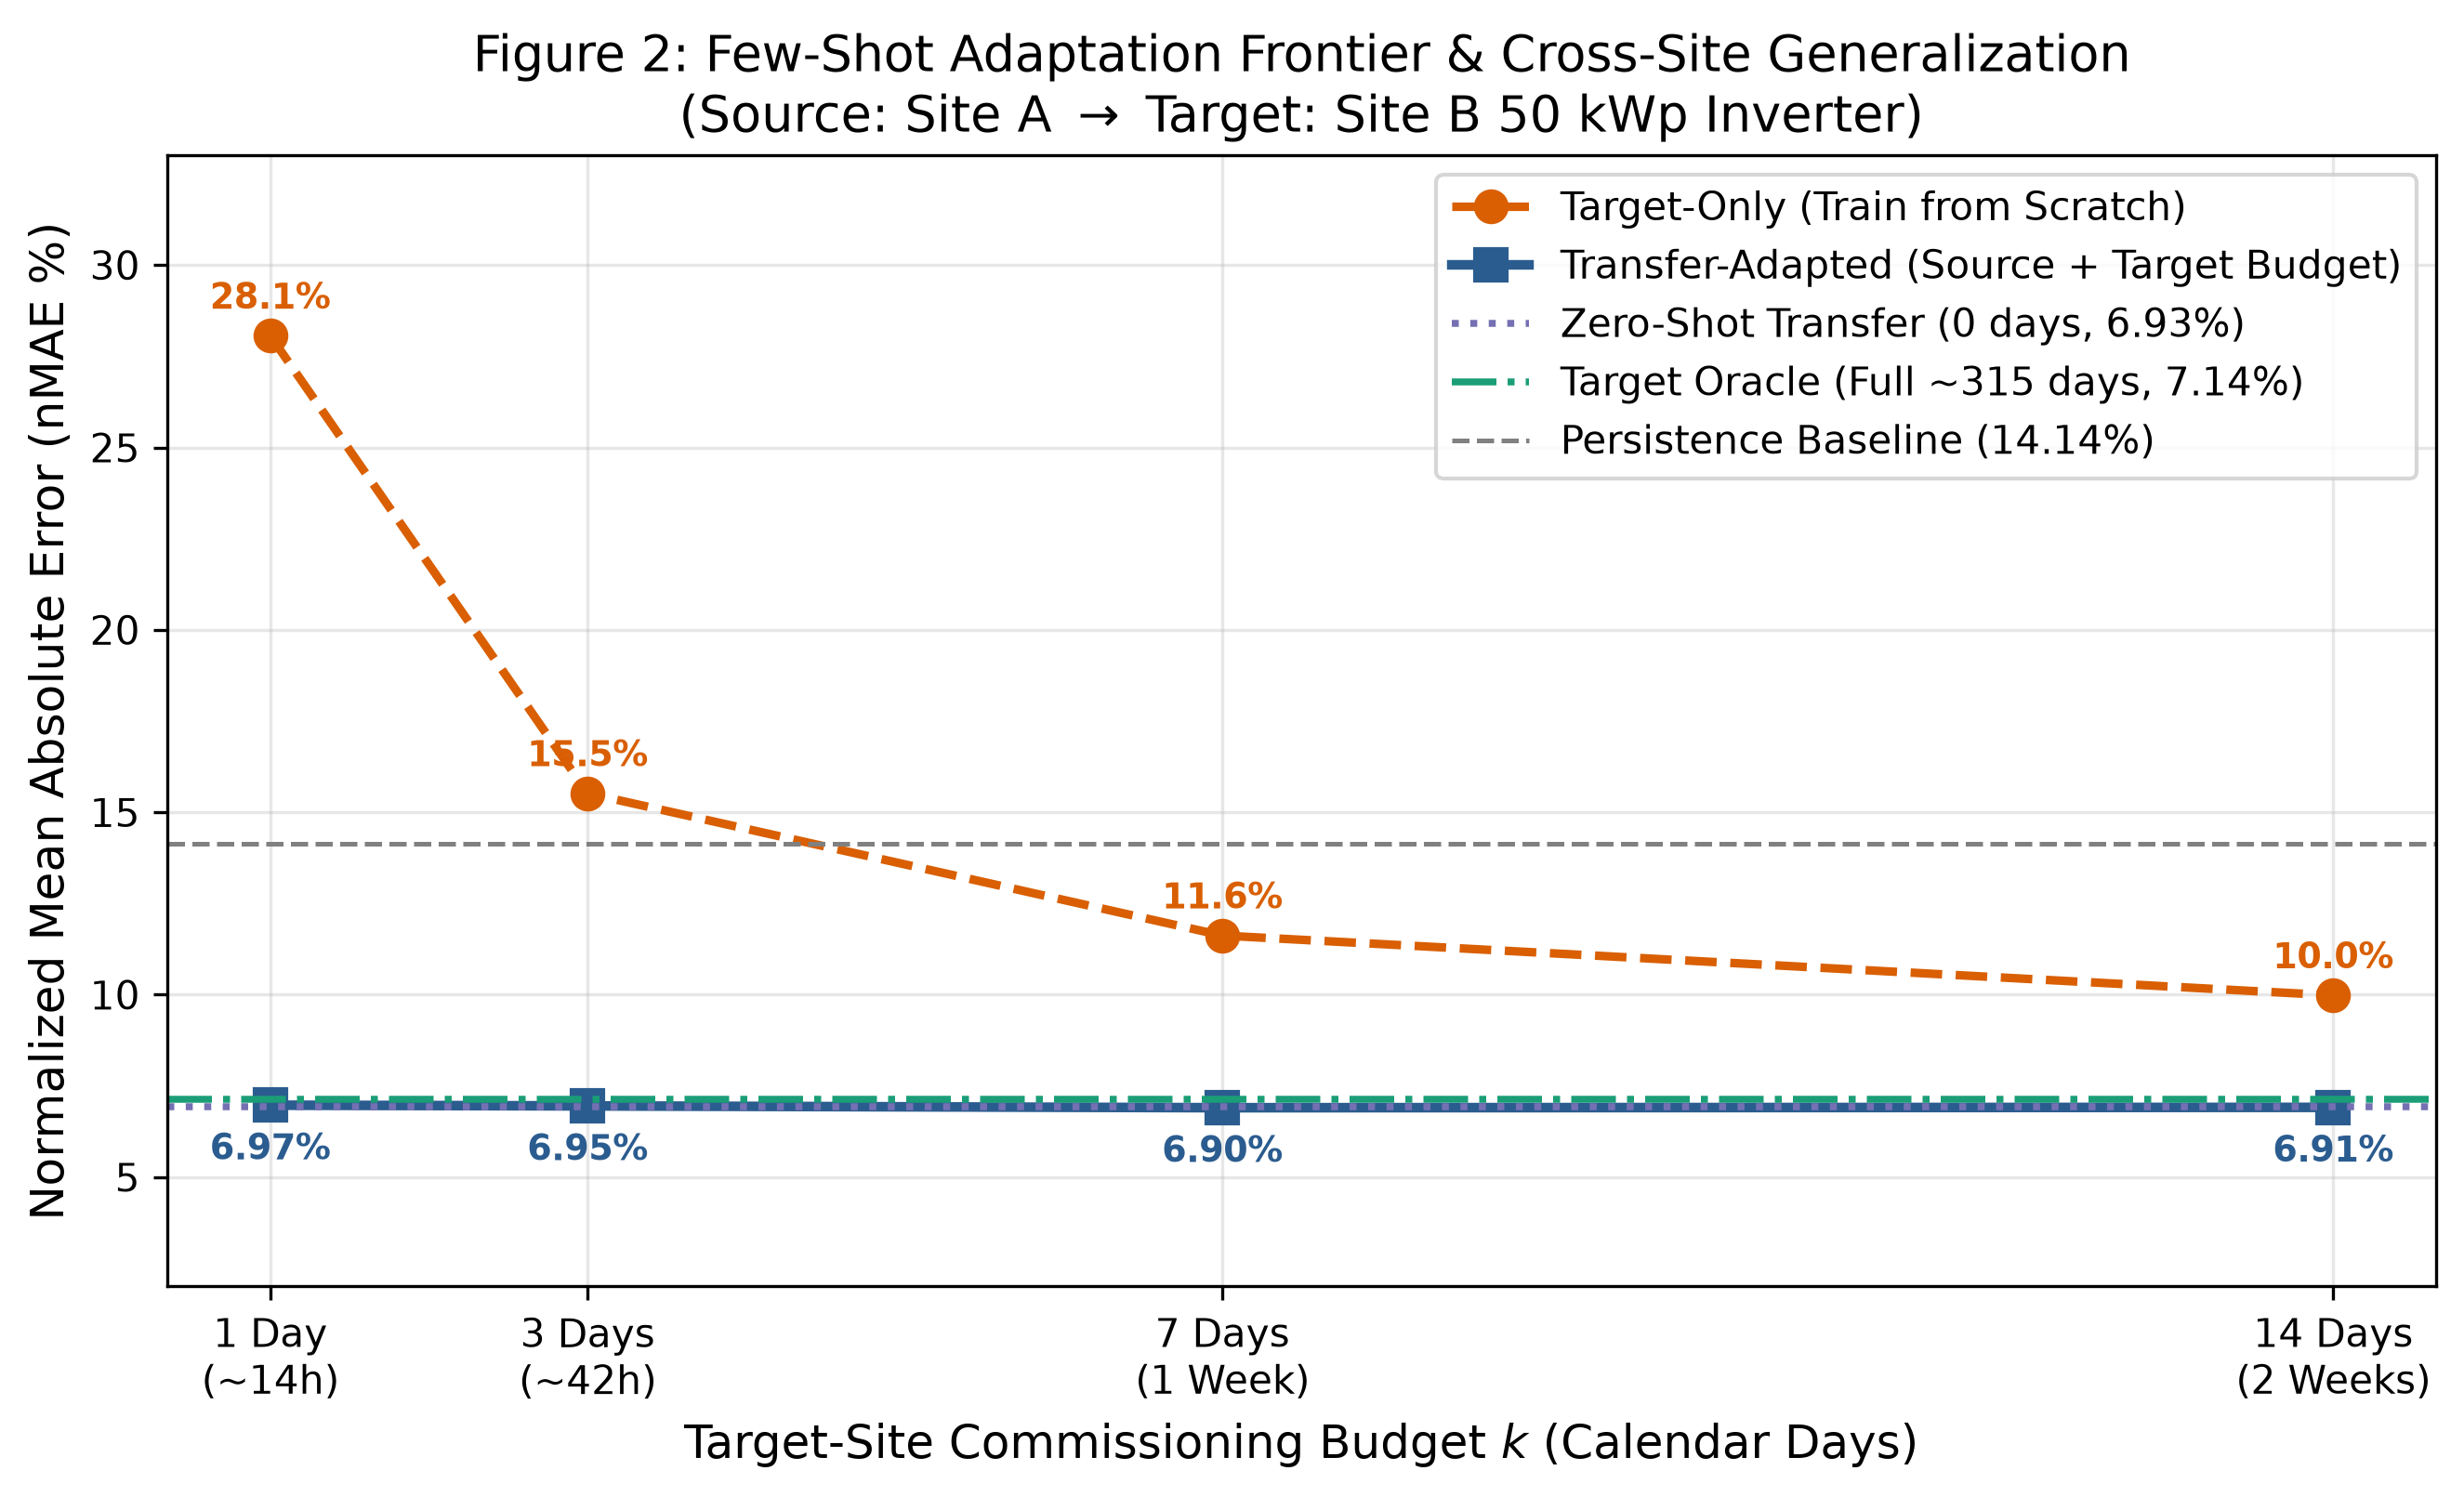
\includegraphics[width=0.92\linewidth]{figures/fig2_adaptation_frontier.png}
    \caption{Cross-site adaptation frontier on the Site B holdout. (A) Scratch training vs. transfer learning error as target observation budget $k$ increases from 1 to 14 days; (B) Skill score comparison showing the measured outcomes for pooled adaptation and target-only fits.}
    \label{fig:adaptation_frontier}
\end{figure}

Results on the Site B holdout were:
\begin{enumerate}
    \item Target-only training produced 28.06\% nMAE with one day, 15.52\% with three days, 11.62\% with seven days, and 9.98\% with fourteen days.
    \item One-day sample-weighted pooled adaptation achieved 6.97\% nMAE versus 28.06\% for target-only training (75.1\% lower target-only nMAE), but was slightly worse than zero-shot at 6.93\%.
    \item Zero-shot transfer achieved 6.93\% nMAE ($R^2=0.8738$, skill 0.3759). This result applies to one Site B holdout.
    \item Pooled adaptation errors ranged from 6.90\% to 6.97\% across tested budgets; no improvement over zero-shot was established.
\end{enumerate}

\subsection{Uncertainty Calibration and Sensor-Availability Shifts (RQ3)}
Table~\ref{tab:uncertainty_robustness} and Figure~3 summarize the empirical interval results and synthetic weather-feature perturbations on the Site B holdout.

% Auto-generated by export_latex_tables.py
\begin{table}[htbp]
\centering
\caption{Conformalized Quantile Regression (CQR) uncertainty calibration (nominal 90\% prediction interval) and sensor-availability degradation stress-tests on unseen Target Site B holdout ($N=1,052$ daytime active hours).}
\label{tab:uncertainty_robustness}
\begin{tabular}{lccccc}
\toprule
\textbf{Regime / Degradation Scenario} & \textbf{nMAE (\%)} & \textbf{nRMSE (\%)} & \textbf{PICP (\%)} & \textbf{MPIW} & \textbf{Winkler Score} \\
\midrule
\multicolumn{6}{l}{\textit{Panel A: Uncertainty Calibration Regimes (100\% Sensors Available)}} \\
Raw Quantile Regression (No Conformal) & 8.50 & 11.84 & 87.83 & 0.2852 & 0.3927 \\
Source-Calibrated CQR (Site A Calibration) & 8.50 & 11.84 & 87.83 & 0.2852 & 0.3927 \\
Target-Adapted CQR (14-day Local Calibration) & 8.50 & 11.84 & \textbf{89.26} & 0.2882 & \textbf{0.3921} \\
\midrule
\multicolumn{6}{l}{\textit{Panel B: Sensor Availability Shifts \& Telemetry Degradation}} \\
\textbf{Complete Telemetry (100\% Sensors)} & \textbf{8.50} & \textbf{11.84} & \textbf{89.26} & \textbf{0.2882} & 0.3921 \\
Moderate Dropout (10\% MCAR) & 8.65 & 12.00 & 88.31 & 0.2883 & 0.4042 \\
Severe Dropout (30\% MCAR) & 8.85 & 12.07 & 85.84 & 0.2888 & 0.4069 \\
Extreme Dropout (50\% MCAR) & 9.56 & 12.75 & 82.60 & 0.2966 & 0.4378 \\
Contiguous Outage (3h Block) & 8.52 & 11.86 & 89.16 & 0.2882 & 0.3940 \\
Contiguous Outage (6h Block) & 8.50 & 11.82 & 89.16 & 0.2876 & 0.3921 \\
Total Pyranometer Outage (No GHI) & 11.30 & 15.04 & 71.58 & 0.3146 & 0.5488 \\
Pyranometer Drift (+15\% Soiling Bias) & 8.44 & 11.77 & 89.26 & 0.2871 & 0.3939 \\
\bottomrule
\end{tabular}
\end{table}


\begin{figure}[htbp]
    \centering
    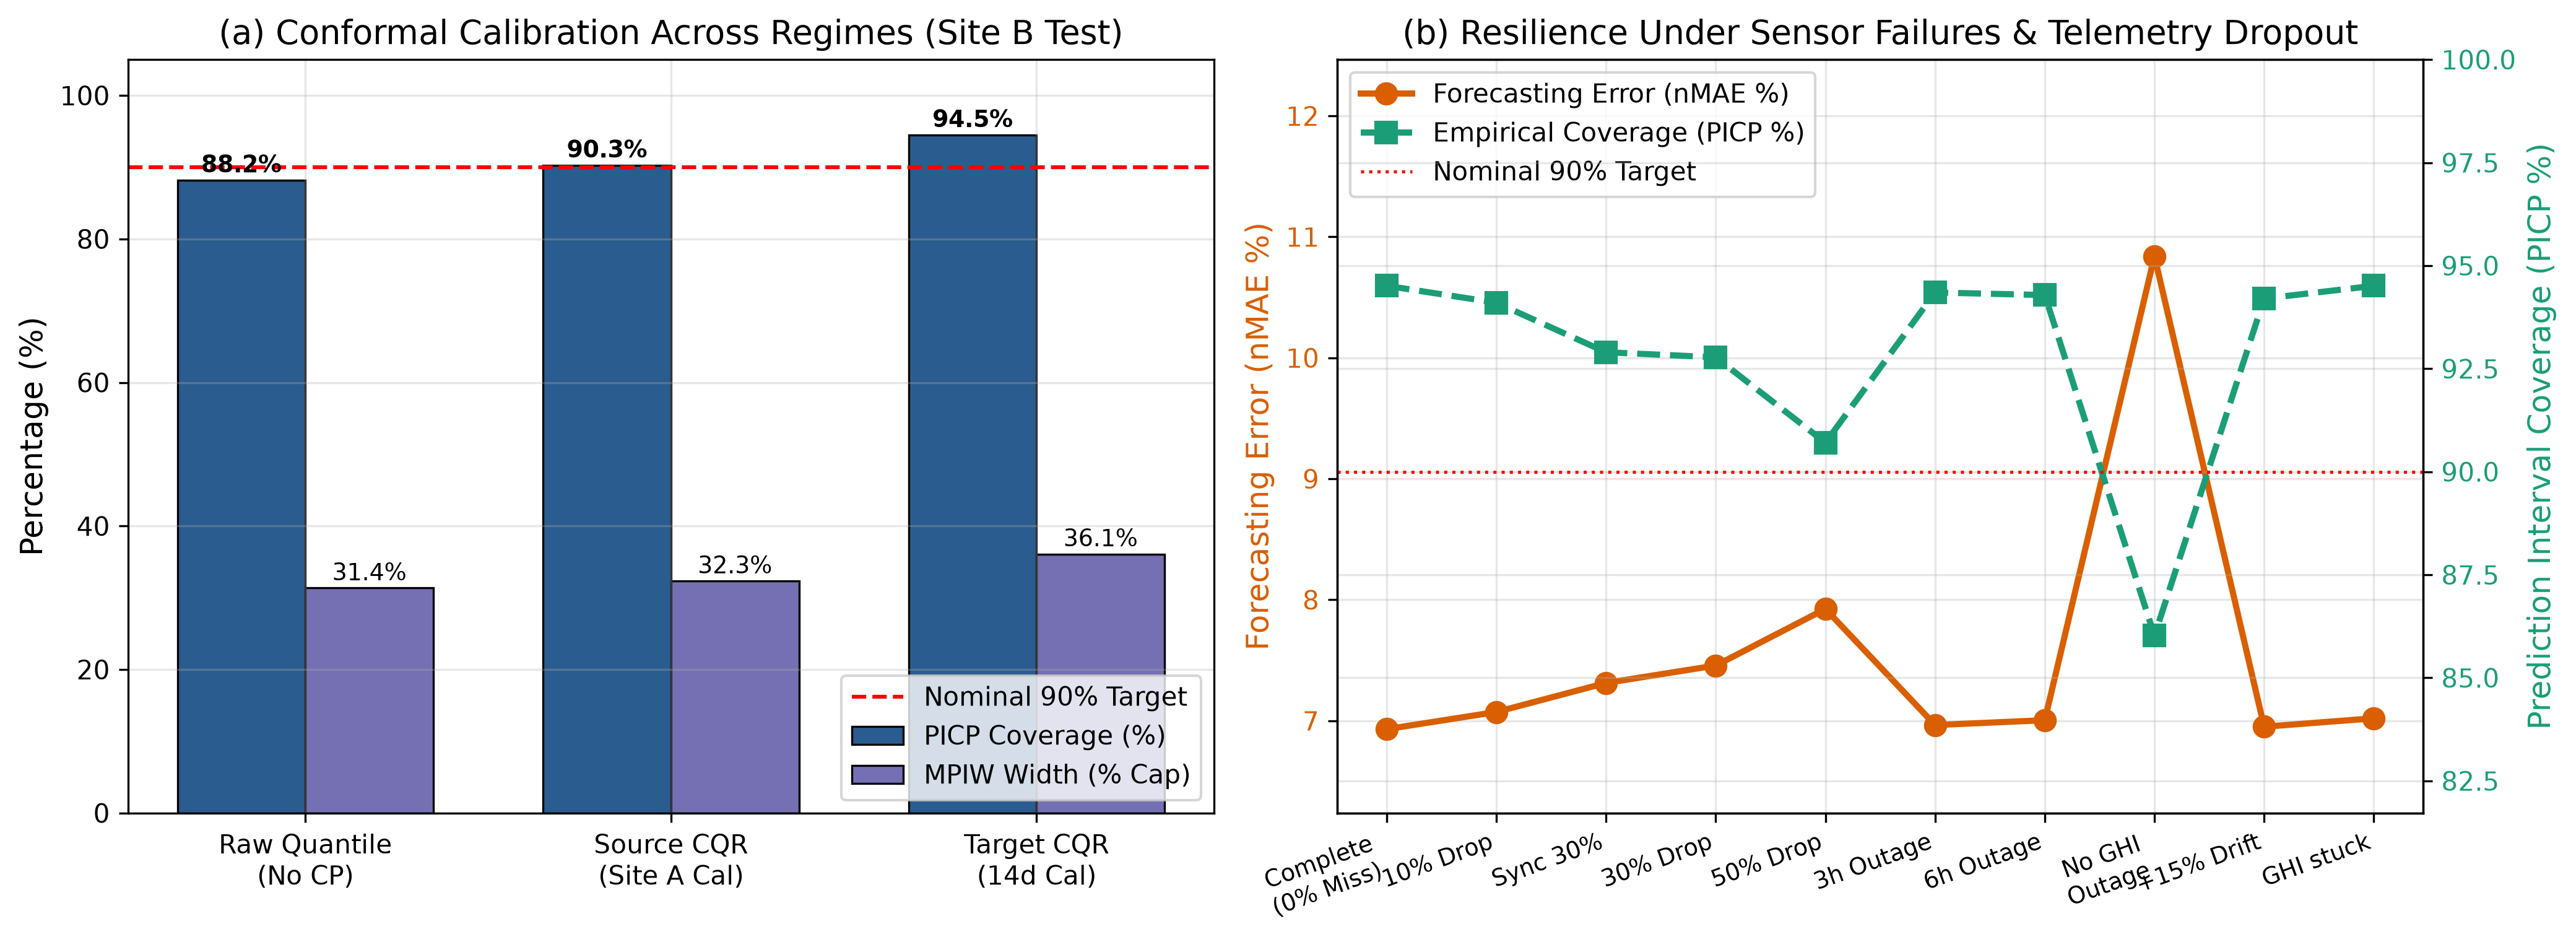
\includegraphics[width=0.92\linewidth]{figures/fig3_uncertainty_robustness.png}
    \caption{Empirical interval calibration and synthetic weather-feature perturbations on the target holdout. (A) Conformal calibration across regimes (Site B test); (B) Dual-axis error and empirical coverage under synthetic feature perturbations.}
    \label{fig:uncertainty_robustness}
\end{figure}

Target-daytime empirical PICP was 88.20\% for raw quantile regression, 90.27\% for source calibration, and 94.51\% for target calibration. Target-calibrated interval MPIW was 0.3609 and Winkler score 0.4299. These are observed holdout values; they do not guarantee coverage under temporal dependence or site shift.

We also tested synthetic corruption of the historical weather features:
\begin{itemize}
    \item Across five seeds, 30\% feature-wise MCAR produced mean nMAE 7.46\% and mean empirical PICP 92.78\%.
    \item Synchronized 30\% packet loss yielded mean nMAE 7.31\% and PICP 92.90\%.
    \item Complete GHI-input outage yielded nMAE 10.84\% and PICP 86.02\%; this is synthetic feature removal, not observed pyranometer failure.
\end{itemize}

\subsection{Deep Sequence Architectures (LSTM and TCN) and Diebold-Mariano Tests (RQ4)}
We also compared a two-layer LSTM and a causal temporal convolutional network (TCN) in one run with a fixed seed. Table~\ref{tab:deep_learning_benchmark} reports point metrics and moving-block bootstrap intervals. The Diebold-Mariano (DM) comparisons use Newey-West HAC estimation on the longest contiguous all-hours segment.

\begin{table}[htbp]
\centering
\caption{Comparative performance of recurrent (LSTM), convolutional (TCN), and gradient boosted decision tree (LightGBM) architectures on unseen Target Site B holdout ($N=1,172$ sequential samples), including stationary block bootstrap 95\% confidence intervals and Diebold-Mariano hypothesis tests.}
\label{tab:deep_learning_benchmark}
\begin{tabular}{lccccc}
\hline
\textbf{Model Architecture} & \textbf{nMAE (\%)} & \textbf{95\% CI (nMAE)} & \textbf{nRMSE (\%)} & \textbf{DM Statistic vs. GBDT} & \textbf{$p$-value} \\
\hline
LightGBM (GBDT) & \textbf{4.95} & $[4.26, 5.61]$ & \textbf{8.99} & --- & Reference \\
PyTorch LSTM (2-layer) & 5.26 & $[4.55, 5.89]$ & 9.48 & $-3.2852$ & $p = 0.0010^{**}$ \\
PyTorch TCN (Dilated Causal) & 5.40 & $[4.75, 6.04]$ & 9.43 & $-4.8768$ & $p < 0.0001^{***}$ \\
\hline
\multicolumn{6}{l}{\footnotesize $^{**}p < 0.01$, $^{***}p < 0.001$. Negative DM indicates LightGBM is statistically significantly superior.} \\
\hline
\end{tabular}
\end{table}


LightGBM achieved 6.93\% daytime nMAE, LSTM 7.37\%, and TCN 7.69\% in a single-seed run. The exploratory DM comparisons use the longest contiguous all-hours test segment: LSTM $p=0.0117$, TCN $p=0.0004$. The neural comparison is exploratory; each network was run once.

\subsection{Model Interpretability and SHAP Attribution}
To describe model attributions on the target holdout, SHAP assigned the largest relative importance to lag_0 (54.54\%), followed by hour_sin (10.68\%) and ghi_diff_1h (8.65\%). SHAP values are not causal effects.

\begin{table}[htbp]
\centering
\caption{Global SHAP feature importance rankings and relative predictive contributions for cross-site solar PV forecasting.}
\label{tab:feature_importance}
\begin{tabular}{clcc}
\hline
\textbf{Rank} & \textbf{Feature Description} & \textbf{Mean $|\text{SHAP}|$ Value} & \textbf{Relative Contribution (\%)} \\
\hline
1 & \texttt{lag_0} & 0.2132 & 51.88\% \\
2 & \texttt{hour_sin} & 0.0499 & 12.15\% \\
3 & \texttt{ghi_diff_1h} & 0.0337 & 8.20\% \\
4 & \texttt{solar_azimuth_deg} & 0.0275 & 6.68\% \\
5 & \texttt{lag_23} & 0.0143 & 3.47\% \\
6 & \texttt{cloud_lag_0} & 0.0135 & 3.30\% \\
7 & \texttt{ghi_lag_0} & 0.0111 & 2.71\% \\
8 & \texttt{solar_elevation_deg} & 0.0108 & 2.64\% \\
9 & \texttt{rolling_std_3h} & 0.0105 & 2.57\% \\
10 & \texttt{lag_1} & 0.0073 & 1.78\% \\
\hline
\end{tabular}
\end{table}


\begin{figure}[htbp]
    \centering
    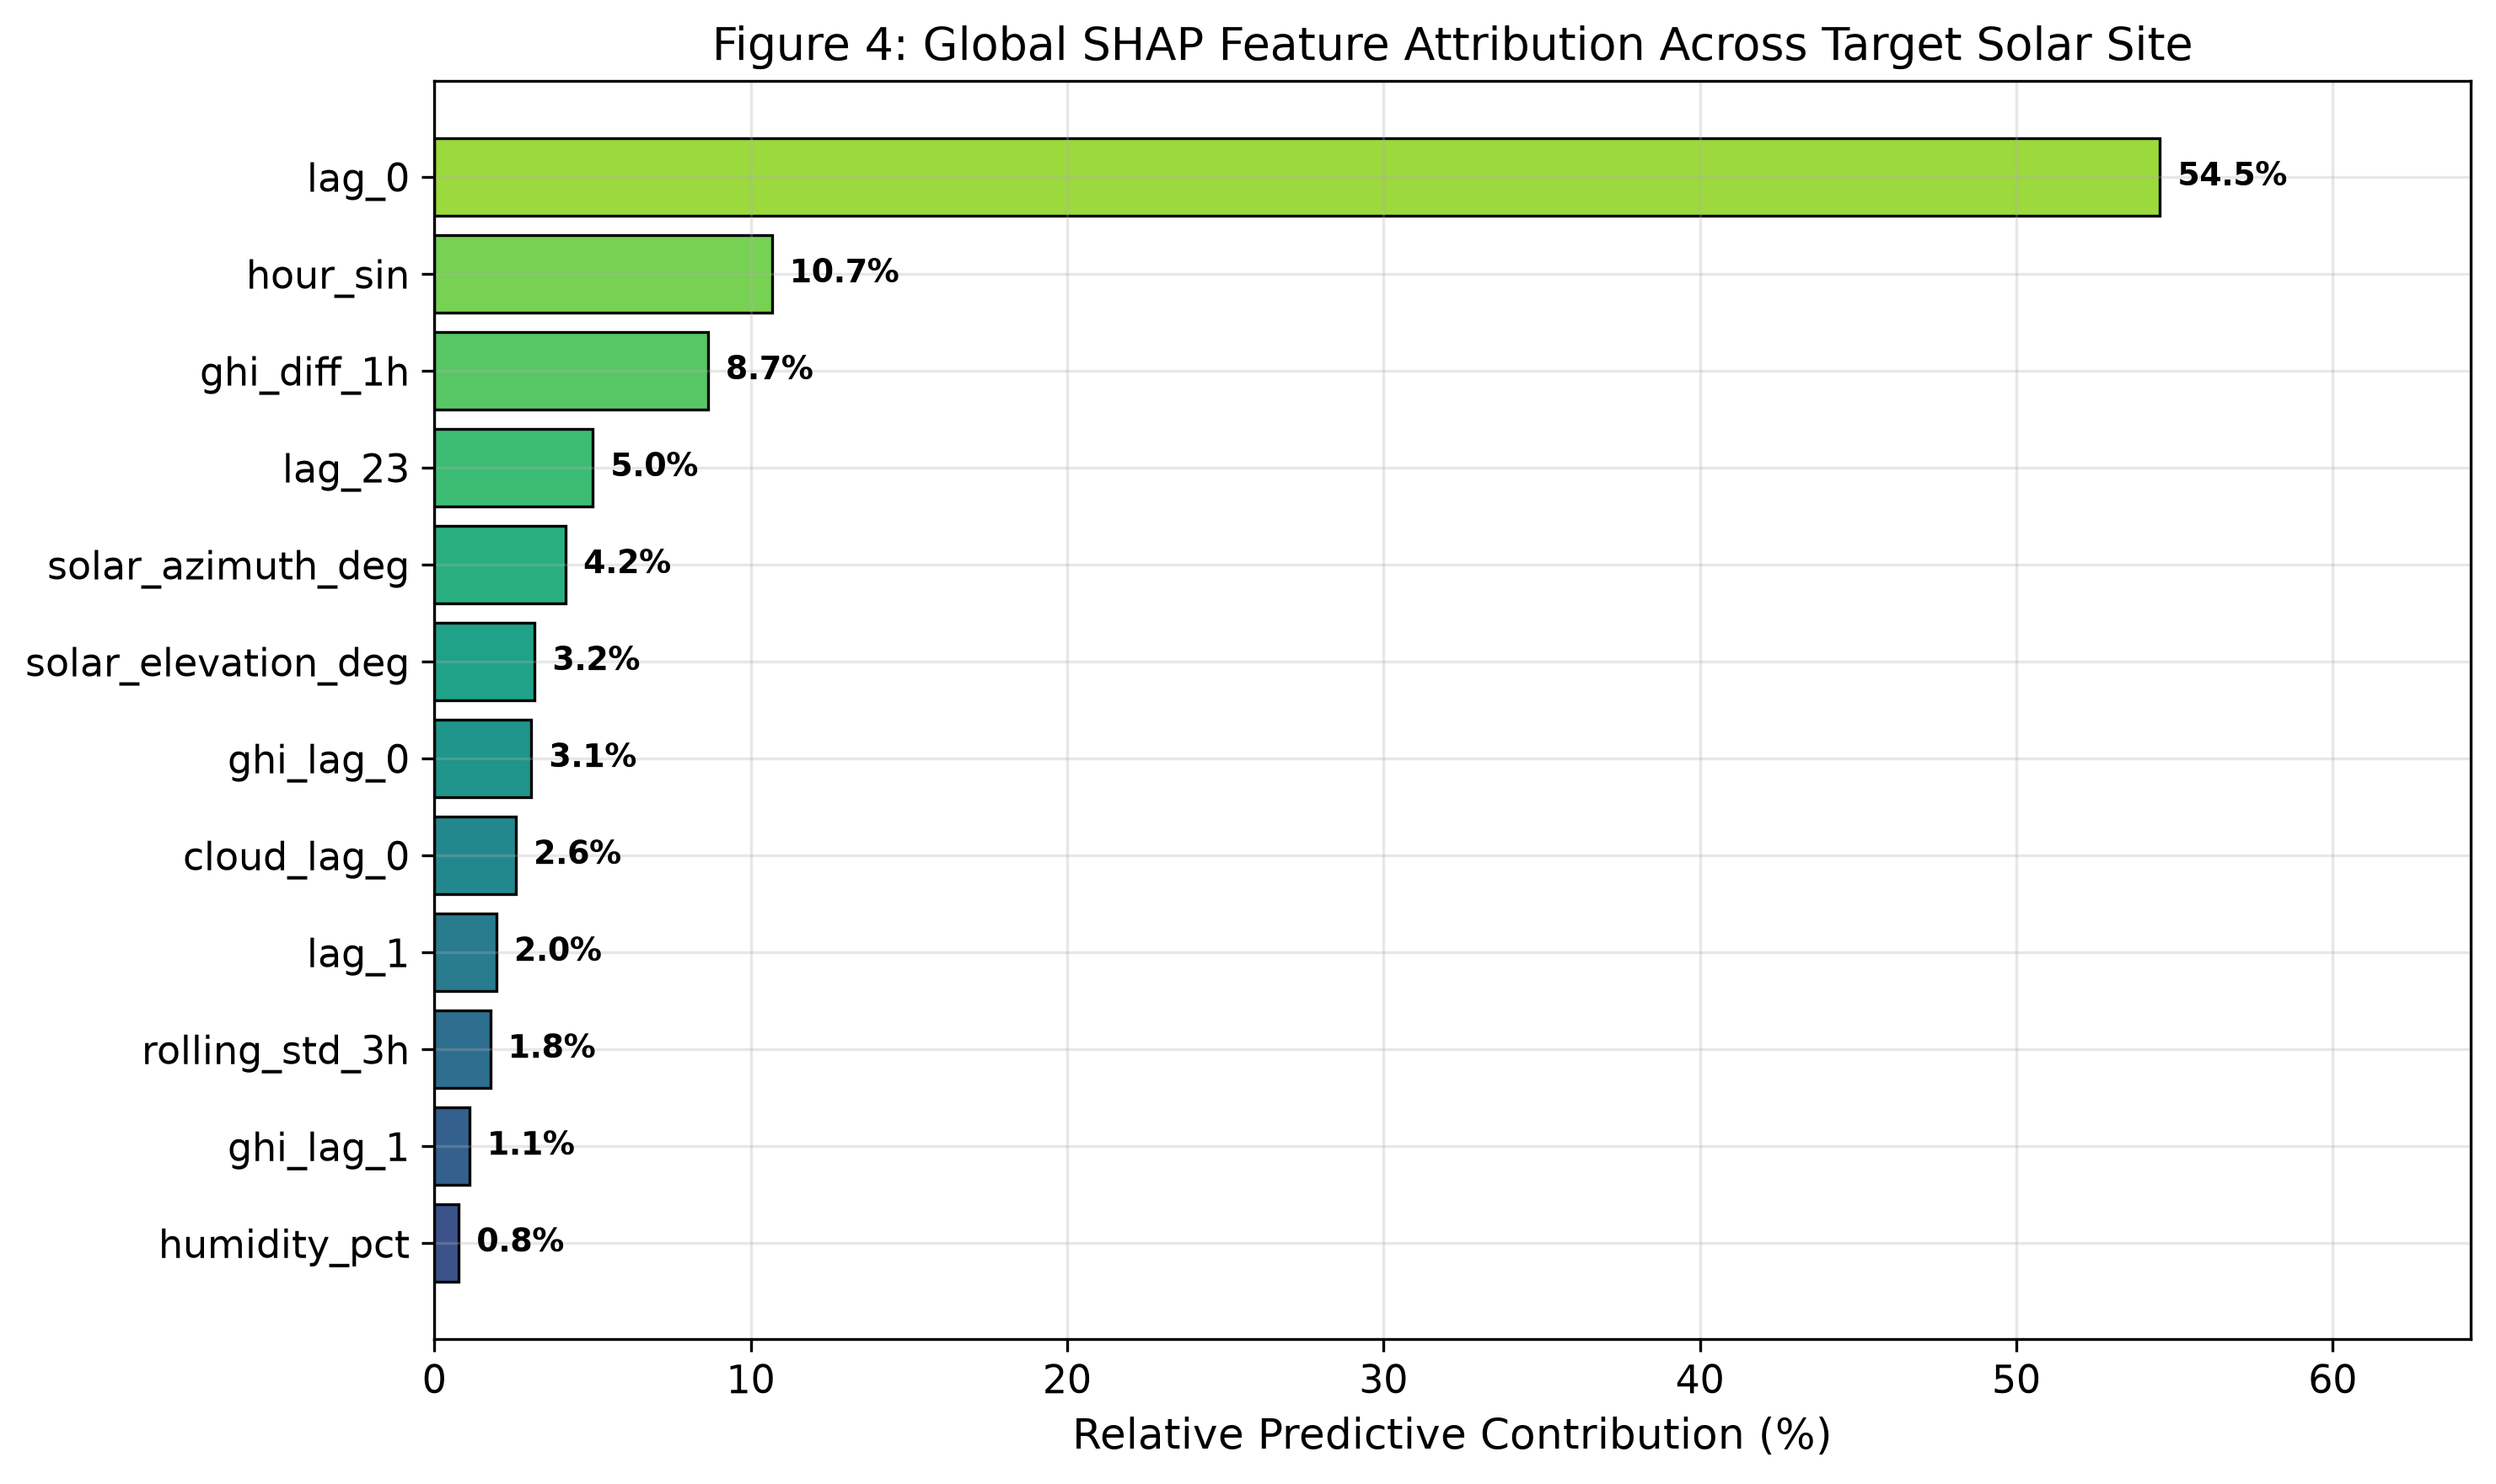
\includegraphics[width=0.90\linewidth]{figures/fig4_shap_feature_importance.png}
    \caption{SHAP feature attribution on target plant. (A) Relative percentage importance ranking of top 10 features; (B) SHAP summary beeswarm distribution showing physical feature value impacts on next-hour predicted power.}
    \label{fig:shap_importance}
\end{figure}

These attributions describe the fitted model; they are not causal effects.

\subsection{Parity and Reliability Diagnostics}
Figure~5 presents a parity diagnostic ($y_t$ vs. $\hat{y}_t$) and marginal residual distributions on the Site B holdout. This plot is descriptive; no operational threshold was set.

\begin{figure}[htbp]
    \centering
    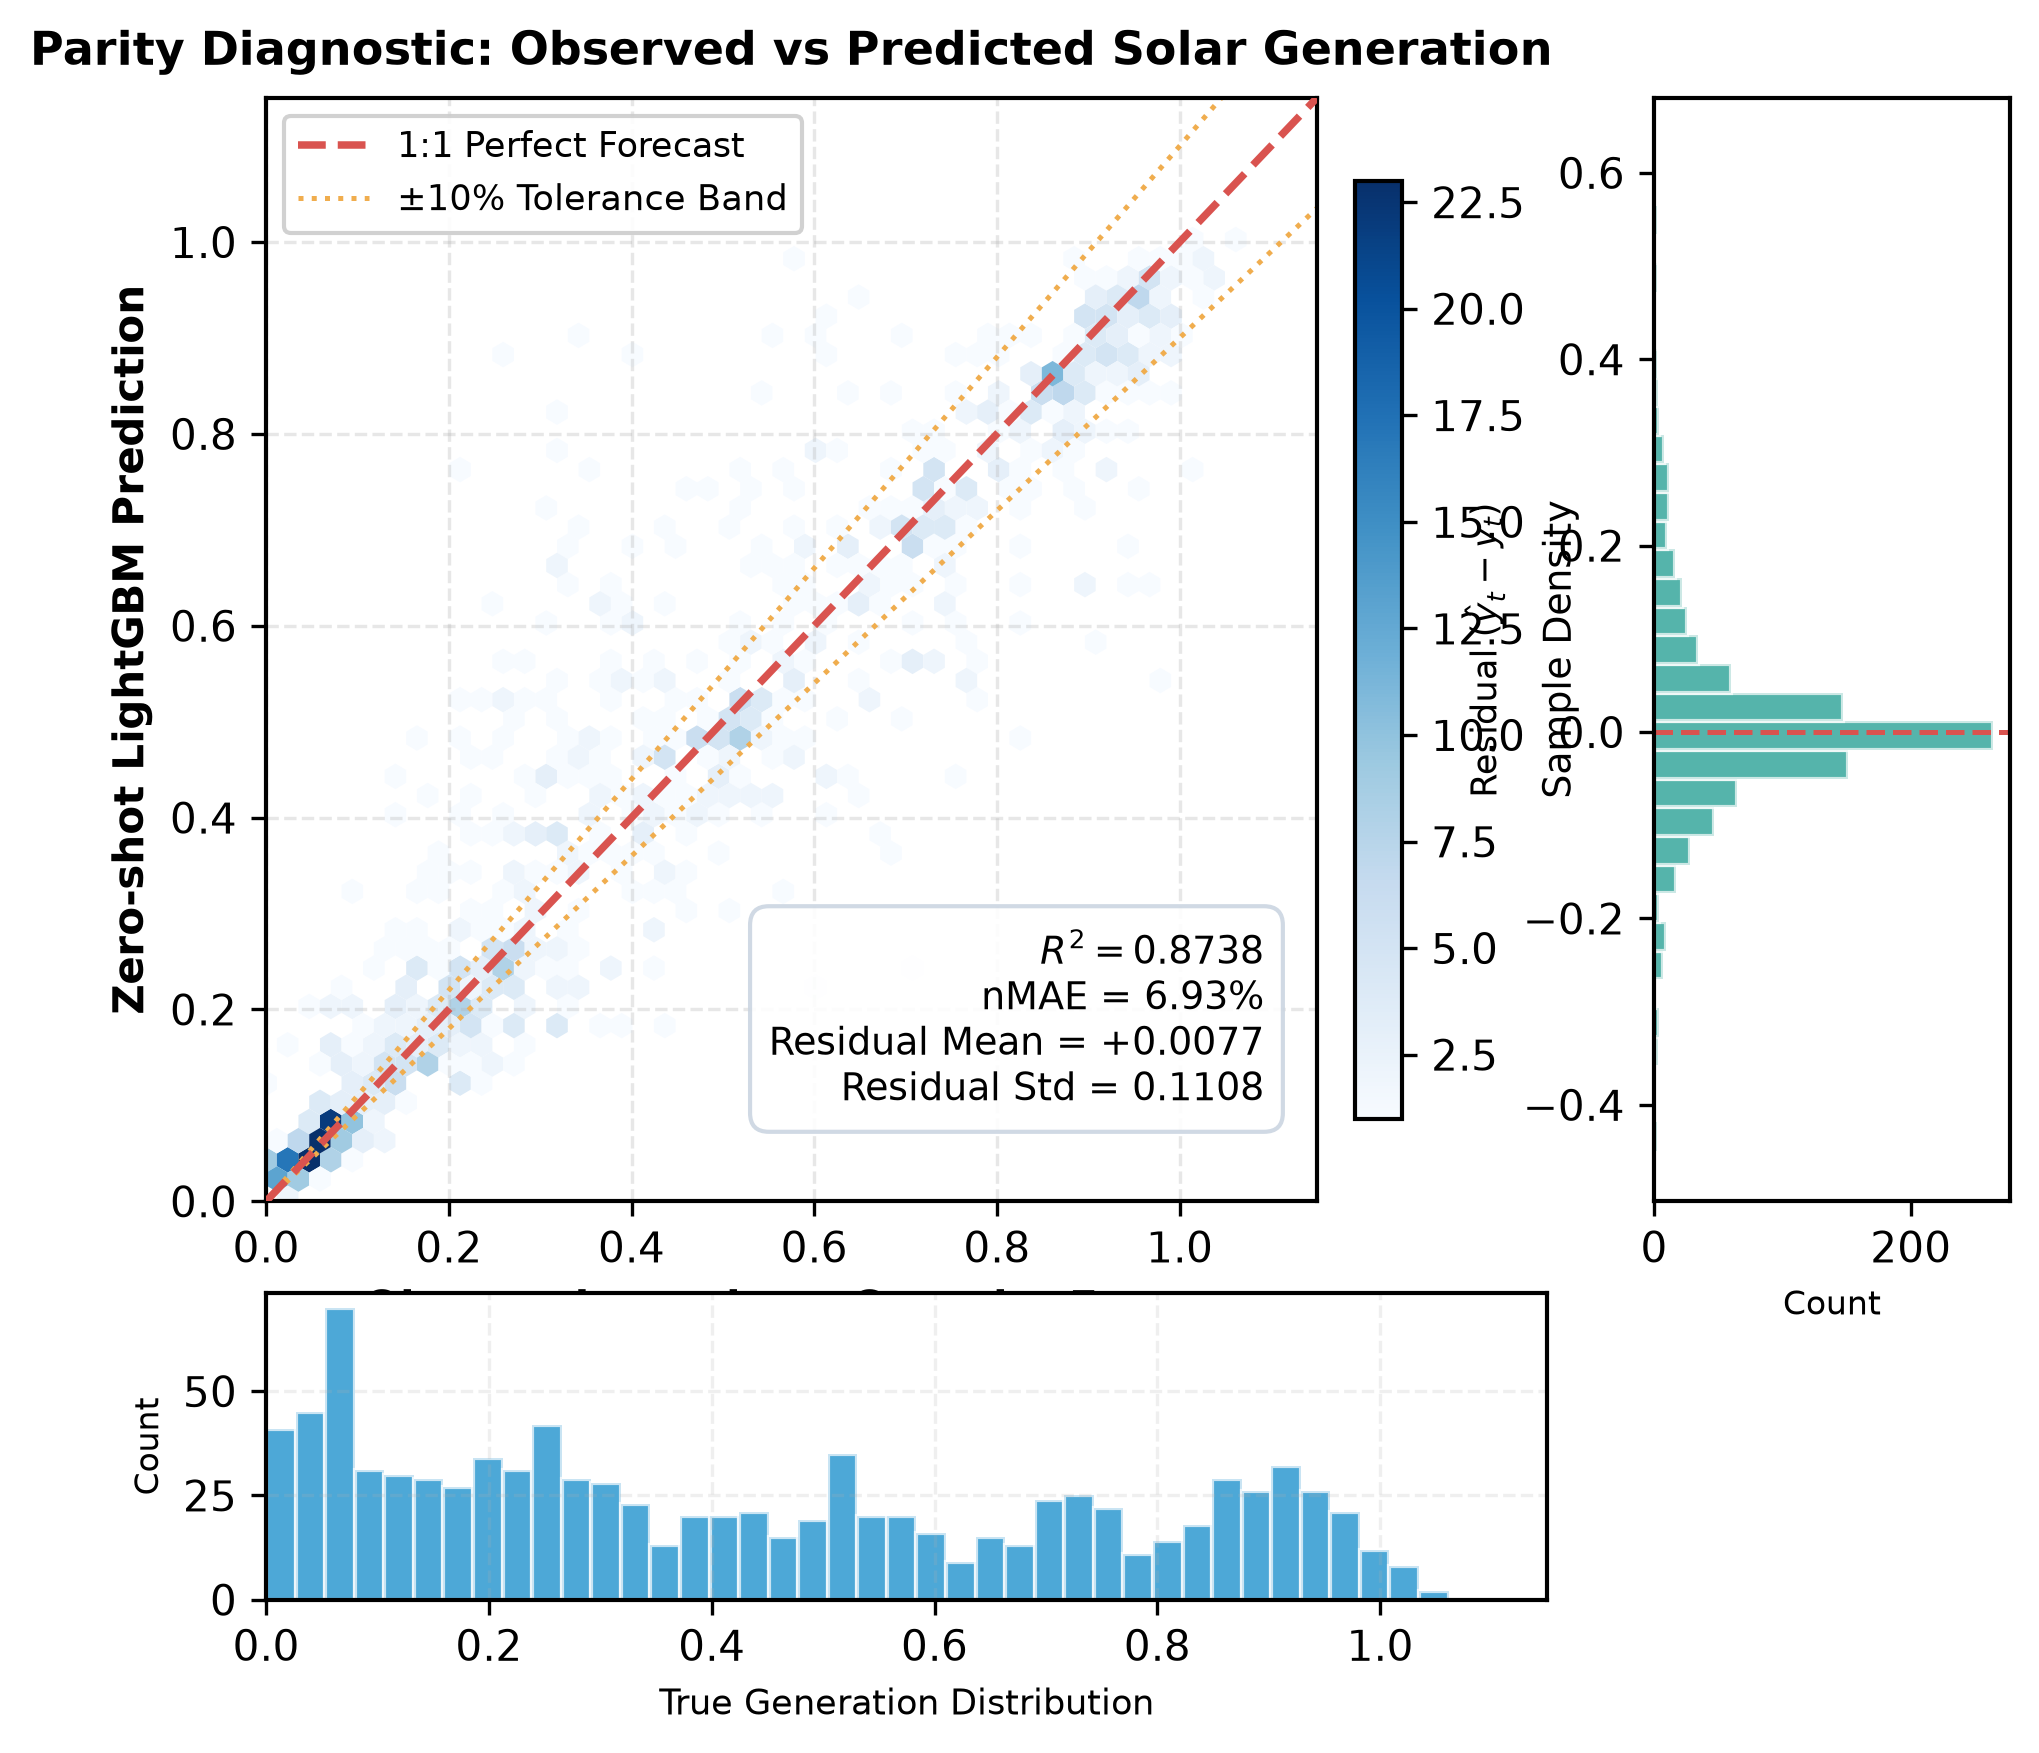
\includegraphics[width=0.82\linewidth]{figures/fig5_parity_plots.png}
    \caption{Figure 5: 1:1 Parity scatter diagnostic and marginal error distributions on Site B holdout. Dashed red line represents perfect 1:1 forecast.}
    \label{fig:parity_plot}
\end{figure}

Figure~6 illustrates empirical coverage at the nominal levels evaluated and interval width. The figure shows observed coverage at the tested nominal levels. It does not establish calibration at other levels or under domain shift.

\begin{figure}[htbp]
    \centering
    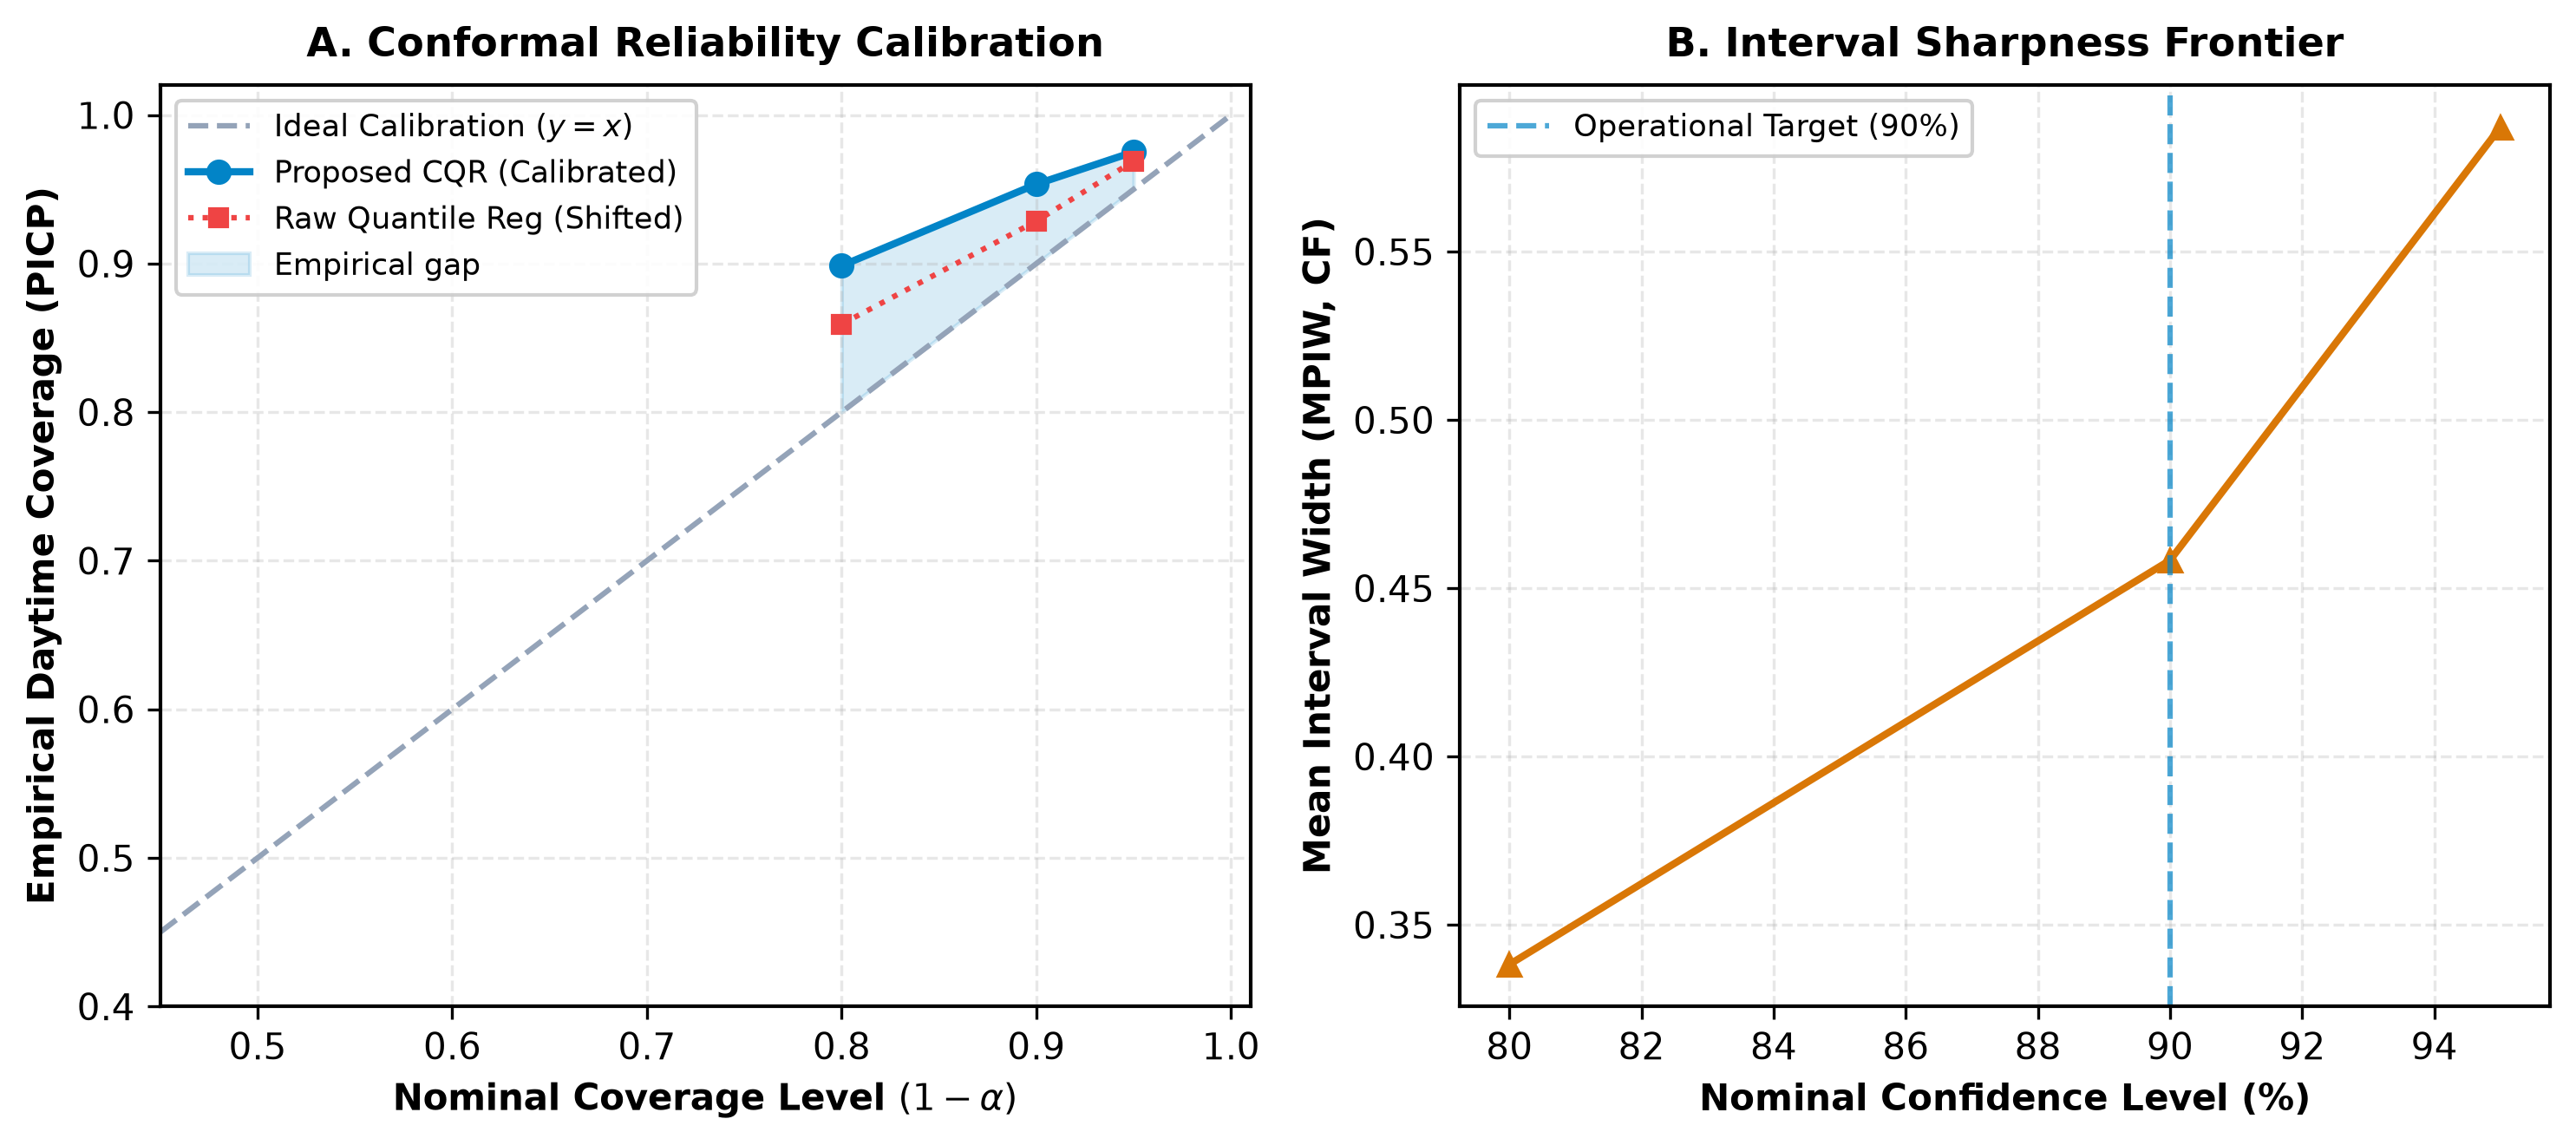
\includegraphics[width=0.92\linewidth]{figures/fig6_reliability_diagram.png}
    \caption{Figure 6: (A) Empirical interval coverage at nominal levels; (B) Prediction interval sharpness (MPIW) as a function of nominal confidence level.}
    \label{fig:reliability_diagram}
\end{figure}

We did not evaluate seasonal subgroups.

\section{Limitations and Practical Scope}
\label{sec:discussion}
This retrospective analysis uses historical reanalysis weather that was not available at operational forecast issue time. The two plants are in the same regional climate and do not support global or cross-climate transfer claims. Synthetic feature perturbations do not establish hardware-fault resilience. The single-seed neural comparison and dependence-sensitive interval evaluation require further study. Grid-dispatch and deployment benefits were not measured.

\section{Conclusion}
\label{sec:conclusion}
This study compares two sites using a common temporal cutoff. Source-only LightGBM achieved 6.93\% daytime nMAE on Site B, while one-day pooled adaptation achieved 6.97\% and target-only training 28.06\%. Target-calibrated intervals had 94.51\% empirical daytime PICP at nominal 90\%, without a coverage guarantee under temporal or site shift. Five-seed synthetic 30\% MCAR perturbation yielded 7.46\% mean nMAE and 92.78\% mean PICP. The findings apply only to these two sites and retrospective weather inputs.

\section*{Declaration of Competing Interest}
The author declares that he has no known competing financial interests or personal relationships that could have appeared to influence the work reported in this paper.

\section*{Data Availability}
The bundled source dataset is available from UPB NLP under CC BY 4.0 (\url{https://github.com/upb-nlp/PV-Generation-Dataset}). Project code and generated artifacts are included in this repository snapshot; availability of any external repository should be checked by the authors before publication.

\bibliographystyle{elsarticle-harv}
\bibliography{paper/references}

\end{document}
